\chapter{Introduction}
\label{ch:introduction}

Social networks are nowadays widely used by people, allowing users to
discuss the most different topics and interact with each other. At the same time in these
platforms we are observing an increasing polarization between the users.
This inspired several studies which have been conducted about the topic
\cite{Garimella2018,Guerra2013,conover2011political,gruzd2014investigating},
the most recent ones focusing on COVID-19
\cite{Jiang2021,green2020elusive,jiang2020political,lang2021maskon}
and vaccination \cite{Cossard2020}.

Polarization is the social phenomenon according to which people tend do
separate in opposing communities with few people remaining neutral
\cite{Guerra2013}. A close phenomenon is that of the Echo Chambers, groups in
which people that have the same opinions enforce their respective ideas
\cite{Garimella2018}, a concept very similar to the definition of polarization
as given in \cite{sunstein1999law}: ``group polarization arises when members of
a deliberating group move toward a more extreme point in whatever direction is
indicated by the members' predeliberation  tendency. `[L]ike polarized
molecules, group members become even more aligned in the direction they were
already tending''\cite{turner1987rediscovering}.

In this research we aim at finding a method for detecting Echo Chambers, by
analyzing data retrieved from social medias like Twitter and Reddit: we define
the \acrfull{ECP} and the \acrfull{D-ECP} and propose techniques for solving
and approximating them.

We introduce these new approaches for finding Echo Chambers due to growing complexity and quantity of
online interactions; the last year of social distancing forced
many people to stay at home and consequently we can expect that the time
they spent social medias increased from the past, thus producing a denser
network of interactions.

Our two problems are defined on a signed graph which distinguishes
between \emph{friendly} and \emph{hostile} interactions between the users.
Differently from previous studies of polarization on signed graph
\cite{xiao2020searching}, we define
and incorporate in our problems the ideas of \emph{contents} (the piece of
information which is discussed) and \emph{threads} (the "locality"
discussing a content).

Our idea is that Echo Chambers correspond to subgraphs discussing one or more
controversial topics (which trigger many negative reactions in the network when
seen as a whole) with few or no negative interactions: users in this bubble
agree with each other, thus reinforcing their initial position.

\section{Background}
\label{sec:background}

A \emph{graph} $G = (V, E)$ is a collection of \emph{vertices} or \emph{nodes} $V$ and
\emph{edges} or \emph{links} $E \subseteq V \times V$ between the nodes, representing relationships
between entities. Graphs are very useful in
representing many interesting concepts from social sciences, biology, physics,
chemistry and geography (for example, we can see in
\autoref{fig:tex/img/sample-graph} that they
can be used to represent the users' retweets during US 2010 midterm
elections)\cite{Newman2018,Menczer2020}.

\begin{figure}
	\centering
	\includegraphics[width=0.6\linewidth]{tex/img/sample-graph.png}
	\caption[Retweet network during 2010 midterm elections]{The retweet network of posts regarding US during 2010 midterm
		elections. Red and blue nodes are associated with conservative and
		progressive users, respectively. The picture was taken from
		\cite{Menczer2020}.}
	\label{fig:tex/img/sample-graph}
\end{figure}

\paragraph{Different Types of Graphs}%
\label{par:different_types_of_graphs}

In its simplest form graph are \emph{undirected} and \emph{unweighted}. In an
\emph{undirected} graph relationships are bi-directional, while in directed graph
the order of nodes in a link reflects the
direction (i.e.\ an edge $e_{ij} $ is different from an edge $e_{ji} $). A weighted
graph associates a weight $\omega _e$ to each edge $e \in E$
\cite{Menczer2020,AlbertLaszloNortheasternUniversity2016}.

Sometimes edges are allowed to be either positive or negative: these networks
are usually called \emph{signed graphs}. An acquaintance
network, for example, can be modeled through a signed graph, with negative and
positive edges denoting animosity and friendship, respectively \cite{Newman2018}.

\bigskip

In the rest of the document we will abuse notation and refer to vertices both
as $v_{i} \in V $ and $i \in V$; similarly we will refer to edges both as
$e_{ij} \in E $ and as $ij \in E$.

\bigskip

Representing relationships between entities which span over more than two
dimensions requires the definition of an ever more complex structure, the
\emph{multiplex graph}. A \emph{multiplex graph} is a set of graphs (also
referred to as \emph{layers}) $\{ G_i = (V, E_i)\} _i$ over the same set of
vertices $V$, each $G_i$ having its own set of vertices $E_i \subseteq V \times V $ (an
example can be seen in \autoref{fig:tex/img/multiplex-graph}). Multiplex graphs
can be used, for example, to model temporal networks, where
each \emph{layer} corresponds to a snapshot of the relationship at a certain
point in time \cite{Newman2018}.

\begin{figure}
	\centering
	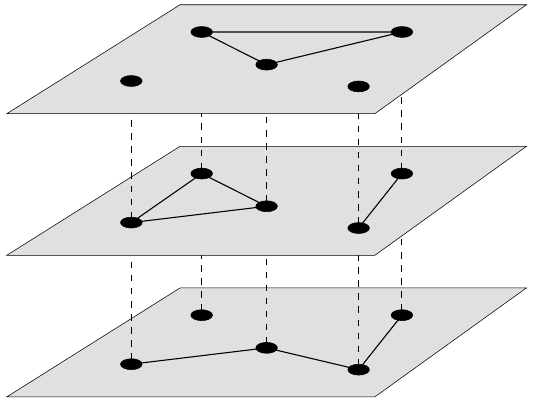
\includegraphics[width=0.4\linewidth]{tex/img/multiplex-graph.png}
	\caption[An example of multiplex graph]{An example of \emph{multiplex
			graph} with three layers. Picture taken from
		\cite{Newman2018}.}%
	\label{fig:tex/img/multiplex-graph}
\end{figure}

\section{Problem}
\label{sec:problem}

In this section, after defining the graph on which the research is
carried out, we give a formal definition of the problems that we
study in the thesis.

\subsection{The Interaction Graph}
\label{sub:interaction-graph}

The \emph{interaction graph} $G$ is the graph we utilize to encode the
information regarding the interactions between the users.

\begin{definition}
	We say that multigraph $G=(V,E^+,E^-)$ is an interaction graph if $G$ is
	directed, weighted and signed with weights in $[-1,+1]$, and $G$ is also a
	multiplex graph.
\end{definition}

In this graph each user is associated to a vertex $v \in V$. For this reason we
will sometimes refer to vertices as users in the rest of the document.

Each edge of the graph corresponds to an interaction: edge $e_{ij}$
going from $v_i$ to $v_j$ represents user $i$ replying to
user $j$. Also, the corresponding weight $w_e$ encodes the \emph{sentiment} of
the interaction: negative and positive values are associated with hostile and
friendly interactions, respectively, with smaller values of $w_e$ being
associated to more hostile interactions.

% Each edge is associated to an interaction between the incident users: the
% the orientation is used to encode which user replied (an edge $e_{ij}$ means
% that user $v_i$ replied to user $v_j$). The weight encodes the animosity of the
% interactions, so that an edge with weight $< 0$ corresponds to a negative
% interaction

% $G = (V, E^{+}, E^{-})  $ is a
% signed and weighted graph, the weights being in the interval $[-1, +1]$,
% corresponding to positive and negative interactions, meaning that for smaller
% values of the weight the interaction will more "negative".

% The \emph{interaction graph} is also directed, so that an edge from vertex $v_{i}
% $ to vertex $v_{j} $ corresponds to a reply from user $v_{i} $ to $v_{j} $.

Let a content $C$ be any kind of resource that triggers a discussion in one or
more threads $T$, where a thread can be any social media post sharing the content $C$. The set of threads associated to $C$ is denoted as
$\mathcal{T}_{C} $. A content is usually represented by a newspaper article and
it is identified by its URL, e.g.

	{\footnotesize
		\begin{center}
			\url{https://www.nytimes.com/2021/03/04/us/richard-barnett-pelosi-tantrum.html}
		\end{center}
	}

A corresponding thread then may be, for example, the one generated by a user
posting and commenting the same URL on its Twitter account (see
\autoref{fig:twitter-thread}), thus generating a discussion.

\begin{figure}
	\centering
	
\includegraphics[width=0.6\linewidth]{tex/img/twitter_thread.png}
	\caption[Thread-content distinction example from Twitter]{A thread
		associated to the mentioned New York Times article.}%
	\label{fig:twitter-thread}
\end{figure}

In our \emph{interaction graph} each layer is associated
to a thread $T$ whose edges are the interactions happening in it.
Note that since it is a multigraph, each of the layers can contain more than one
edge between two users, as each pair of users can reply to each other more than
one time.

We will also use $\mathcal{C} $ for denoting the set of contents.

An example of an \emph{interaction graph} can be seen in
\autoref{fig:interaction-graph-example}.

\begin{figure}
	\begin{center}
		\begin{subfigure}[b]{0.3\textwidth}
			\centering
			\tikzfig{tex/tikz/graph_thread1}
			\caption{$T_{1} \in \mathcal{T}_{C_{1}} $}
			\label{fig:tex/tikz/graph_thread1.tikz}
		\end{subfigure}
		\begin{subfigure}[b]{0.3\textwidth}
			\centering
			\tikzfig{tex/tikz/graph_thread2}
			\caption{$T_{2} \in \mathcal{T}_{C_{1}} $}
			\label{fig:tex/tikz/graph_thread2.tikz}
		\end{subfigure}
		\begin{subfigure}[b]{0.3\textwidth}
			\centering
			\tikzfig{tex/tikz/graph_thread3}
			\caption{$T_{3} \in \mathcal{T}_{C_{2}} $}
			\label{fig:tex/tikz/graph_thread3.tikz}
		\end{subfigure}
	\end{center}
	\caption[Example of an \emph{interaction graph}]{An example of an \emph{interaction graph}, green and red edges
		representing positive and negative interactions with weights $-1$ and
		$+1$, respectively. It
		contains three threads ($T_1$, $T_2$ and $T_3$) and two contents ($C_1$
		and $C_2$), the first two layers each being
		associated to a thread of content $C_{1} $, the last layer to a thread
		of content $C_{2} $.}
	\label{fig:interaction-graph-example}
\end{figure}

\subsection{The Problem Definition}%
\label{sub:the_problem_definition}

The main goal of the research is finding echo chambers in social medias, more
specifically on the \emph{interaction graph} as defined in
\autoref{sub:interaction-graph}.

Our definition is based on the idea that echo chambers can be identified by
looking at contents which are highly debated (we will call
this type of content \emph{controversial}) but which are discussed with little
or no animosity in some subgraphs. These subgraphs are the \emph{Echo
	Chambers}.

\bigskip

Given an \emph{interaction graph} $G = (V, E^{+}, E^{-})$ on some contents
$\mathcal{C} $ and threads, let $E^{+}_k$ and $E^{-}_k$ be the set of
positive and negative edges associated to thread $T_k$, respectively. We define
$\eta(T)$ to be the ratio between the number of
negative edges and the total number of edges in the layer associated to thread
$T$, i.e.
\begin{equation*}
	\eta(T_k) = \frac{|E^{-}_{k}|}{|E^{-}_{k}| + |E^{+}_{k}|}.
\end{equation*}

Now, for a content $C$, let $E^{+}_l = \cup_{T_k \in \mathcal{T} _C} E^+_k$ and $E^{+}_l = \cup_{T_k \in \mathcal{T} _C} E^+_k$.
Similarly to $\eta(T)$, $\eta(C)$ is defined as the fraction of negative edges associated to
content $C$, i.e.
\begin{equation*}
	\eta(C_l) = \frac{|E^{-}_{l}|}{|E^{-}_{l}| + |E^{+}_{l}|}.
\end{equation*}

\begin{definition}[Controversial thread]
	Let $\alpha \in [0,1]$. A thread (or content) is \emph{controversial} if
	$\eta(T) > \alpha$ (or, similarly, $\eta(C) > \alpha $). Conversely, a
	thread (or content) is \emph{non-controversial} if $\eta(T) \leq \alpha$
	($\eta(C) \leq \alpha$).
\end{definition}

Intuitively, \emph{controversial} threads contain many negative
interactions. We denote as $\hat{\mathcal{C} } \subseteq \mathcal{C} $ the
set of \emph{controversial} contents.

\medskip

\emph{Echo Chambers} correspond to \emph{non-controversial} subgraphs
(i.e.\ with few negative edges) discussing a
\emph{controversial} content.

More formally, for a set of vertices $U \subseteq V$, let $T[U]$ be the subgraph induced in the layer associated to
thread $T$; let $|T^{+} [U]|$ and $|T^{-} [U]|$ be its number
of positive and negative edges, respectively.

We define $\mathcal{S}_C (U)$ as the set of \emph{non-controversial} threads
induced by $U$, for \textit{controversial} contents $C \in \mathcal{\hat{C}}$, i.e.
	{\small
		\begin{equation}
			\mathcal{S}_C (U) = \{ T[U] \; s.t. \; T[U] \; non\text{-}controversial, T \in \mathcal{T} _{C}, U \subseteq V\}.
		\end{equation}
	}

Thus, $\mathcal{S}_C (U)$ will contain threads which are \emph{locally}
non-controversial but it is defined only for contents that are \emph{globally}
controversial.

\medskip

We now define the Echo Chamber Score of a set of vertices $U$.

\begin{definition}[Echo Chamber Score]
	Let $U \subseteq V$ be a subset of vertices. Its \emph{Echo Chamber Score}
	$\xi(U)$ is

	\begin{equation}
		\label{eq:echo-chamber-score}
		\xi(U) = \sum^{}_{\mathcal{C} \in \mathcal{\hat{C}}} \sum^{}_{T[U] \in
		\mathcal{S} (U)} (|T^{+} [U]| - |T ^{-} [U]|).
	\end{equation}
\end{definition}

We can now define the \acrfull{ECP}.

\begin{problem}[\acrfull{ECP}]
Given an \emph{interaction graph} $G$ and $\alpha \in [0, 1]$ find a set of vertices $U \subseteq
	V$ maximizing the Echo Chamber Score \eqref{eq:echo-chamber-score}.
\end{problem}

We will denote with $\hat{U}$ the set of users maximizing
\eqref{eq:echo-chamber-score} and with $\xi(G)$ its corresponding score, i.e.

\begin{align*}
	\hat{U} & \coloneqq \argmax_{U \subseteq V} \xi(U), & \xi(G) & \coloneqq
	\xi(\hat{U}).
\end{align*}

\subsection{The Densest Echo Chamber Problem}%
\label{sub:the_densest_echo_chamber_problem}

The \acrshort{ECP} does not take into account the number of users producing a
certain score; this means that the set $U$ may involve also very sparse
subgraphs, depending on the structure of the graph $G$.

For this reason it is interesting also to study another variant of the
\acrshort{ECP}, the \acrfull{D-ECP}, which we now define.

\begin{definition}[Densest Echo Chamber Score]
	Let $U \subseteq V$ be a subset of vertices. Its \emph{Densest Echo Chamber Score}
	$\psi(U)$ is

	\begin{equation}
		\label{eq:densest-echo-chamber-score}
		\psi(U) = \sum^{}_{\mathcal{C} \in \mathcal{\hat{C}}} \sum^{}_{T[U] \in
		\mathcal{S} (U)} \frac{(|T^{+} [U]| - |T ^{-} [U]|)}{|U|}.
	\end{equation}
\end{definition}

Similarly to the \acrshort{ECP} we can now define the corresponding problem

\begin{problem}[\acrfull{D-ECP}]
Given an \emph{interaction graph} $G$ and $\alpha \in [0, 1]$ find a set of vertices $U \subseteq
	V$ maximizing the Densest Echo Chamber Score \eqref{eq:densest-echo-chamber-score}.
\end{problem}

Note that $\psi(U) = \xi(U) / |U|$. The solutions to this problem are, in a certain sense, a \emph{stronger} concept of Echo
Chambers: we look for a group of vertices $U$ whose
score $\xi(U)$ is high when compared to $|U|$, i.e.\ a smaller subgraph with a
large $\xi(U)$ will be preferred over a much bigger and sparser subgraph, even
if the latter achieves an higher Echo Chamber Score.

\section{Goals}
\label{sec:goals}

This work addresses the following research questions:

\begin{enumerate}
	\item How can we solve the \acrlong{ECP} and the \acrlong{D-ECP}?
	\item Are they solvable or approximable in polynomial time?
	\item Are these definitions capable of finding echo chambers in real world
	      data?
\end{enumerate}

We will show that these problems are not approximable in polynomial time within
some non-trivial factor and present different methods for solving and
approximating them. We will validate one of the presented approximation
algorithms over synthetic and real-world data, and see that, while in the first
case it is able to reconstruct subgraphs whose vertices have many positive edges, in
the second one it fails to recognize communities.

\section{Structure of the thesis}
\label{sec:structure-thesis}

The thesis is structured as follows:

\begin{enumerate}
	\item \autoref{ch:background} presents previous works and concepts
	      needed for the development of the methods presented in
	      the following chapters.
	\item \autoref{ch:complexity} provides proofs regarding the approximability
	      of \acrshort{ECP} and \acrshort{D-ECP}.
	\item \autoref{ch:solving} defines methods for solving
	      and approximating the \acrshort{ECP} and \acrshort{D-ECP} problems.
	\item \autoref{ch:resultsAndAnalysis} focuses on analyzing the
	      data, how it is retrieved and preprocessed, and discussing the results
	      obtained by applying the introduced methods.
	\item \autoref{ch:conclusionsAndFutureWork} presents the positive effects
	      and the drawbacks of the results, as well as possible future
	      developments and improvements.
\end{enumerate}

\section{About the Thesis}
\label{sec:about-thesis}

The Python code used to obtain the results presented in the rest of the
document is available at the following URL

\begin{center}
	\url{https://github.com/morpheusthewhite/master-thesis}
\end{center}
